
\chapter{Week2}

\section{Monday}\index{Monday_lecture}
\subsection{Logistic equations}
\[\frac{\diff p}{\diff t}=p(a-bp)
\]
where $a$ is intrinsic equation, $\frac{a}{b}$ is carrying capacity, and $p_0$: the initial population $=p(0)$.
\[\int\frac{\diff p}{p(a-bp)}=\int\diff t
\]
\[\dots
\]
\[\frac{p}{|a-bp|}=e^{at+c}
\]
In order to get away from absolute value we need to separate the initial value into different cases.
\begin{enumerate}
\item
$p_0=\frac{a}{b}$ 
$\left.  \begin{gathered}
\frac{\diff p}{\diff t}=p(a-bp)	\\
p(0)=p_0
\end{gathered}\right\}.\Rightarrow P(t)\equiv P_0$
By uniqueness.
\item
 $P_0<\frac{a}{b}$ Then we can get away from absolute value. However, here comes the question;\\
Why $p_t$ never reaches $\frac{a}{b}$? (Uniqueness)\\%If $P(T)=\frac{a}{b}$ for some $T$, $P(t)\equiv\frac{a}{b}$
\[\frac{p}{a-bp}=\tilde{c}e^{at}, \tilde{c}=\frac{P_0}{a-bP_0}(=e^c)
\]
\[\begin{aligned}
P=&(a-bp)\tilde{c}e^{at}\\
=&a\tilde{c}e^{at}-b\tilde{c}pe^{at}
\end{aligned}
\]
\[p(1+b\tilde{c}e^{at})=a\tilde{c}e^{at}\]
\[p=\frac{a\tilde{c}e^{at}}{1+b\tilde{c}e^{at}}\]
Move the upper $\tilde{c}e^{at}$ down and pluge $\tilde{c}$ in;
\[p=\frac{a}{b+\frac{a-bP_0}{P_0}e^{-at}}
\]
\item
$P_0>\frac{a}{b}$
\[\frac{P}{-(a-bP)}=\frac{P_0}{-(a-bP_0)}e^{at}
\]
\dots$\boxed{P(t)=\frac{a}{b+\frac{a-bp_0}{p_0}e^{-at}}\rightarrow\frac{a}{b}}$ as $t\rightarrow\infty$.

\end{enumerate}


Question:$\left \{	\begin{gathered}
\frac{\diff p}{\diff t}=p(a-bp)	\\
p(0)=p_0
\end{gathered}\right.$ At time $s$, $P(s)=P_s$, for $P$ is a dummy variable, we can write a another linear DE; \[\left \{	\begin{gathered}
\frac{\diff q}{\diff t}=q(a-bq)	\\
q(0)=p_s
\end{gathered}\right.\]
For the solution of those two linear DEs, is $P(t)=q(t-s)$?

\begin{proof}
From above disscussion, we know that the solution of these two DE is:
\[P(t)=\frac{a}{b+\frac{a-bP_0}{P_0}e^{-at}}
\]
\[q(t-s)=\frac{a}{b+\frac{a-bq_0}{q_0}e^{-a(t-s)}}
\]
With the second equation of second DEs; $q(0)=p_s$
\[q(t-s)=\frac{a}{b+\frac{a-bP_s}{P_s}e^{-a(t-s)}}\dots(1)
\]
\[P_s=P(s)=\frac{a}{b+\frac{a-bP_0}{P_0}e^{-a(s)}}
\]
Substitude $P_s$ into (1), we get;
\[q(t-s)=\frac{a}{b+\frac{a-bP_0}{P_0}e^{-at}}=P(t)
\]
\end{proof}
\begin{remark}
This question shows that the solution of the linear differential equations is unique regardless of time (when the time start).
\end{remark}


\begin{example}
A commercial fish population is estimated to have carrying capacity 10,000kg of certain kind of fish. Suppose the annual growth of the total fish population is governed by $\frac{\diff p}{\diff t}=p(1-\frac{p}{10,000})$ and initially there are 2,000kg fish.
\begin{enumerate}
\item[(1)]
What is the fish population after 1 year?Suppose, after waiting for a certain period of time, the owner of the fishery decide to harvest 2,400kg of annually at a constant rate.
\item[(2)]
What is the differential equations governing the fish population now?
\item[(3)]
Draw  the slope field of the equation in (2).
\item[(4)]
What is the minimal waiting period you would recommand to the owner (before harvesting)?
\end{enumerate}
\emph{Answer:}
\begin{enumerate}
\item[(1)]
\[\frac{\diff p}{\diff t}=p(1-\frac{p}{10000})
\]
\[\int\frac{\diff p}{p(1-\frac{p}{10000})}=\int\diff t
\]
\[\frac{1}{p(1-\frac{p}{10000})}=\frac{A}{P}+\frac{B}{1-\frac{P}{1000}}=\frac{A(1-\frac{p}{10000})+BP}{p(1-\frac{p}{10000})}=\frac{A+(B-\frac{A}{10000}P)}{p(1-\frac{p}{10000})}
\]
Then substitude $A=1$, $B=\frac{1}{10000}$ to the second equation;
\[\rightarrow\int(\frac{1}{p}+\frac{\frac{1}{10000}}{1-\frac{p}{10000}})\diff p=t+c
\]
\[lnp-ln(1-\frac{p}{10000})=t+c
\]
\[ln\frac{p}{1-\frac{p}{10000}}=t+c
\]
\[\frac{p}{1-\frac{p}{10000}}=e^{t}e^c\qquad\dots(1)
\]
(1) is the equation shows relation between fish population and time,now substitude the initial value into  it, it means when $t=0$;
\[\frac{2000}{1-\frac{2000}{10000}}=e^c=2500
\]
Substitude it back to (1),
\[p=(1-\frac{p}{10000})2500e^t
\]
We can get the formula of fish population.
\[p=\frac{2500e^t}{1+\frac{1}{4}e^t}
\]
\[\frac{\diff p}{\diff t}=\frac{p}{1-\frac{p}{10000}}-2400
\]
\[p=\frac{2500e^t}{1+\frac{1}{4}e^t}
\]
\item[(2)]
\[\frac{\diff p}{\diff t}=p(1-\frac{p}{10000})-2400
\]
\item[(3)]
\[\begin{aligned}\frac{\diff p}{\diff t}&=p-\frac{p^2}{10000}-2400\\
&=\frac{-1}{10000}(p^2-10000p+24000000)\\
&=\frac{-1}{10000}(p-4000)(p-6000)
\end{aligned}
\]
Now we can draw the slope field:
\begin{figure}[H]
\centering
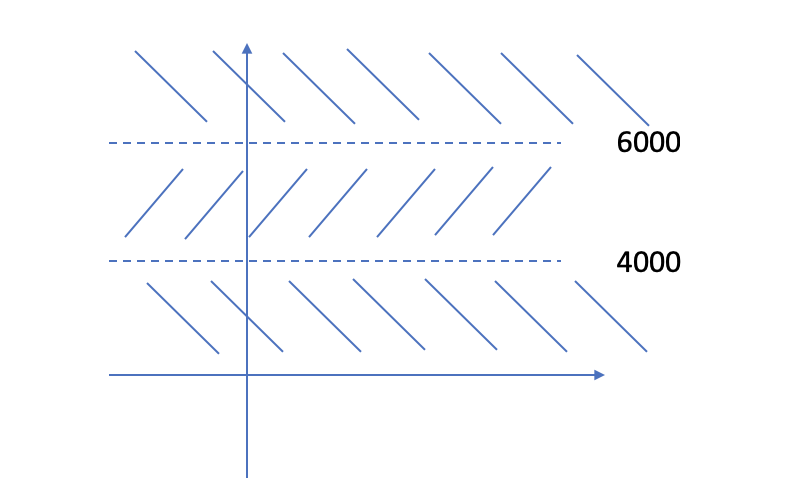
\includegraphics[width=6cm]{week2_Monday}
\caption{Slope field}
\end{figure}
\item[(4)]
One year. From calculation, after one year the population of fish is around 4046 ( $P(1)$) which is greater than 4000. This implies the number of fish wouldn't decline as time goes by as we can see from slope field.
\end{enumerate}
\end{example}



\section{Monday-tutorial}
\paragraph{Newton's Cooling Law}
The rate of change of the temperature $T(t)$ of a body immersed in a medium of constant temperature $A$ is proportional to $A-T$; i.e.
\[\frac{\diff T}{\diff t}=k(A-T), \qquad k \text{ a constant}
\]
\[\left \{	\begin{gathered}
\frac{\diff T}{\diff t}=k(A-T)\\
T(0)=T_0
\end{gathered}\right.\]
\[\int{\diff T}{A-T}=\int k\diff t
\]
\[-ln|A-T|=kt+c
\]
\[|A-T|=e^{-c}e^{-kt}
\]
\[\text{At time $t=0$,}\qquad |A-T_0|=e^{-c}
\]\[|A-T|=|A-T_0|e^{-kt}
\]
\begin{enumerate}
\item
$T_0=A$: $\Rightarrow$ $\quad T(t)\equiv A$   $\qquad\forall t\geq 0$
\item
$T_0>A$: $\Rightarrow$ $\quad T(t)>A$     (Never reach $A$, the same reason illustrated in the lecture. In addition, this is only true when it is first order linear DE.)
\[T-A=(T_0-A)e^{-kt}\rightarrow0\qquad \text{as } t\rightarrow \infty
\]
Therefore, $T(t)\rightarrow A$ as $t\rightarrow \infty$.
\item
$T_0<A$: $\Rightarrow$ $\quad T(t)< A$   $\qquad\forall t\geq 0$
\[A-T(t)=(A-T_0)e^{-kt}\rightarrow0\qquad \text{as } t\rightarrow \infty
\]
\end{enumerate}
\begin{example}
temperature of room $A$, temperature of coffe $T_c$, amount of coffee 1, temperature of cream $T_m$, amount of cream $r(\ll1)$, Boy: adds cream at $t=0$, Girl adds cream at $t=10$. Question: whose cream is cooler when they drink at $t=10$?
\emph{Answer:generally girl's}
\begin{proof}
First, let's calculate the temperature of boy's coffee at the beginning:
\[T_b(0)=\frac{T_c+rT_m}{1+r}\]
After tem minutes;
\[T_b(10)=(T_b(0)-A)e^{-10k}+A
\]
Temperature of girl's coffee at the beginning $T_g(0)=T_c$ and after ten minutes:
\[T_g(10)=(T_c-A)e^{-10k}+A
\]
After girl added cream, the temperature of coffee is:
\[T_g^\prime(10)=\frac{T_g(10)+rT_m}{1+r}
\]
Now let's see which one is cooler;
\[\begin{aligned}T_b(10)-T_g^\prime(10)&=(\frac{T_c+rT_m}{1+r}-A)e^{-10k}+A-\frac{(T_c-A)e^{-10k}+A+rT_m}{1+r}\\
&=\frac{r(A-T_m)}{1+r}+e^{-10k}\frac{r(T_m-A)}{1+r}\\
&=\frac{r(A-T_m)}{1+r}(1-e^{-10k})
\end{aligned}
\]

(1)$T_m=A \Rightarrow T_b(10)=T_g^\prime(10)$\\
(2)$T_m<A \Rightarrow T_b(10)>T_g^\prime(10)$\\
(3)$T_m>A \Rightarrow T_b(10)<T_g^\prime(10)$\\
For most cases, the temperature of cream should be less than the temperature of the room, hence, girl's coffee is cooler than boy's.
\end{proof}
\end{example}